
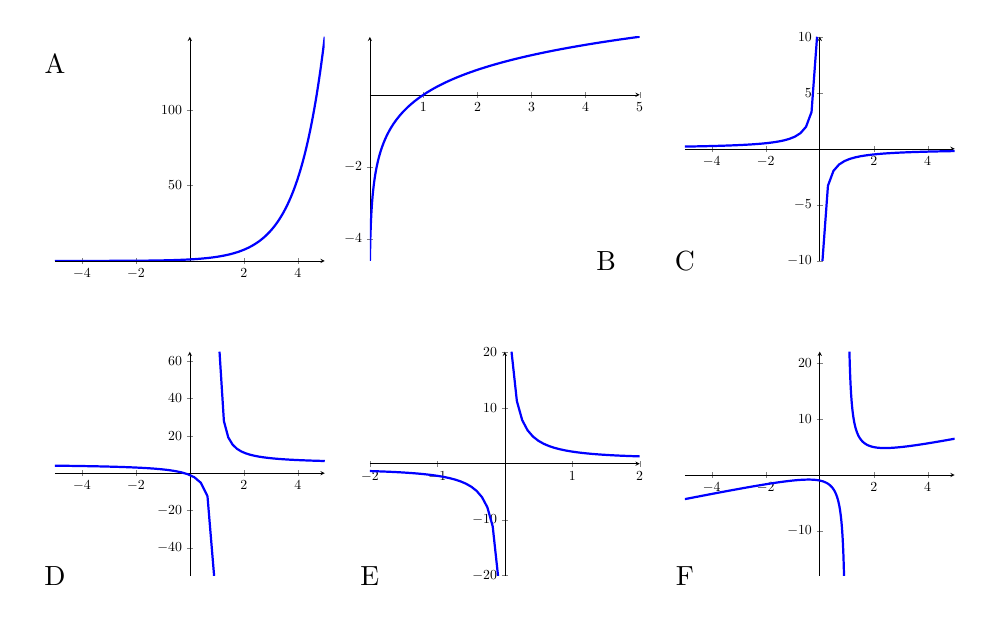
\begin{tikzpicture}[scale=0.5]
    \begin{scope}[shift={(0,0)}]\node[black,circle] at (0,5) {A};
        \begin{axis}[
                axis x line=middle,
                axis y line=middle,
                ]
            \addplot[samples=500, domain=-5:5, blue, ultra thick] {e^x};
        \end{axis}
    \end{scope}
    \begin{scope}[shift={(8,0)}]\node[black,circle] at (6,0) {B};
        \begin{axis}[
                axis x line=middle,
                axis y line=middle,
                ]
            \addplot[samples=500, domain=0.01:5, blue, ultra thick] {ln(x)};
        \end{axis}
    \end{scope}
    \begin{scope}[shift={(16,0)}]\node[black,circle] at (0,0) {C};
              \begin{axis}[
                      axis x line=middle,
                      axis y line=middle,
                      ]
                  \addplot[domain=-5:-0.1, blue, ultra thick] {-1/x};
                 \addplot[domain=0.1:5, blue, ultra thick] {-1/x};
              \end{axis}
    \end{scope}
    \begin{scope}[shift={(0,-8)}]\node[black,circle] at (0,0) {D};
                \begin{axis}[
                        axis x line=middle,
                        axis y line=middle,
                        ]
                    \addplot[domain=-5:0.9, blue, ultra thick] { (5*x+1)/(x-1)};
                \addplot[domain=1.1:5, blue, ultra thick] { (5*x+1)/(x-1)};
                \end{axis}
    \end{scope}
    \begin{scope}[shift={(8,-8)}]\node[black,circle] at (0,0) {E};
         \begin{axis}[
                 axis x line=middle,
                 axis y line=middle,
                 ]
             \addplot[domain=-2:-0.1, blue, ultra thick] { (e^x+1)/(e^x-1)};
         \addplot[domain=0.1:2, blue, ultra thick] { (e^x+1)/(e^x-1)};
         \end{axis}
    \end{scope}
    \begin{scope}[shift={(16,-8)}]\node[black,circle] at (0,0) {F};
           \begin{axis}[
                   axis x line=middle,
                   axis y line=middle,
                   ]
               \addplot[samples=500, domain=-5:0.9, blue, ultra thick] { (x^2+1)/(x-1)};
             \addplot[samples=500, domain=1.1:5, blue, ultra thick] { (x^2+1)/(x-1)};
           \end{axis}
    \end{scope}
\end{tikzpicture}